\documentclass{acm_proc_article-sp}
\usepackage{color}
\usepackage[hyphens]{url}

\def\etal{{\it et al.~}}
\newenvironment{packed_enum}{
\begin{enumerate}
  \setlength{\itemsep}{1pt}
  \setlength{\parskip}{0pt}
  \setlength{\parsep}{0pt}
}{\end{enumerate}}
\newenvironment{packed_item}{
\begin{itemize}
  \setlength{\itemsep}{1pt}
  \setlength{\parskip}{0pt}
  \setlength{\parsep}{0pt}
}{\end{itemize}}


\begin{document}

\title{Risk Perceptions for Wearable Devices}
%\numberofauthors{1}
%\author{
% \alignauthor Linda N. Lee\textsuperscript{1}, Serge Egelman\textsuperscript{1,3}, Joong Hwa Lee\textsuperscript{2}, David Wagner\textsuperscript{1}\\
%   \vspace{0.5em}
%   \affaddr{\textsuperscript{1}University of California, Berkeley, \{lnl,egelman,daw\}@cs.berkeley.edu}, \textsuperscript{2}dlwndghk94@berkeley.edu\\
%   \affaddr{\textsuperscript{3}International Computer Science Institute, egelman@icsi.berkeley.edu}\\
%}

\numberofauthors{1}
\author{
 \alignauthor Anonymous\\
   \vspace{0.5em}
   \affaddr{Some Place}
}
\maketitle
%!TEX root = ../paper.tex

\begin{abstract}
Wearable devices bring great benefits but also new potential privacy and security risks that could expose users' activities without their awareness or consent. Effective design of notifications and security controls for wearable devices will require careful foresight to prevent habituation by treating user attention as a scarce resource, which requires understanding which risks have the potential to be most concerning to users. In this paper, we describe a large-scale survey that we conducted to investigate user security and privacy concerns regarding wearable devices. We surveyed 1,782 Internet users about their perceptions of wearable devices, in order to identify risks that are particularly concerning to users. We specifically controlled for the effects of data type and data recipient on the magnitude of perceived risks, while also collecting open-ended concerns. Finally, we compared wearable device risks to those of more familiar technologies. We hope that this work will inform design of future privacy and security controls for wearable devices.
\end{abstract}

% A category with the (minimum) three required fields
%\category{K.6.5.}{Management of Computing and Information Systems}{Security and protection}[Unauthorized access]

%\terms{Human Factors}{Measurement}{Security}

\keywords{Privacy, Security, User Studies, Risk Perception, Ubiquitous Computing, Wearable Devices} % NOT required for Proceedings
%!TEX root = ../paper.tex

\section{Introduction}

Wearable technologies, or ``wearables,'' are a \$700 million industry \cite{cmo} with a promising future. 52\% of technology consumers are aware of wearables and 33\% are likely to buy one~\cite{NPD}. With 20\% of the general population owning at least one wearable and 10\% using it daily~\cite{WearableStatNews}, wearables are bringing ubiquitous computing to everyday life. Wearable devices enable many benefits, ranging from interaction with virtual objects in an augmented reality world to healthier, fitness-data inspired lifestyles. 

However, wearable devices also bring new potential privacy and security risks that could expose users' activities without their awareness or consent. Although wearable devices are still in their infancy, we have already seen manifestations of these risks. Fitbit's default privacy settings inadvertently exposed information about some of their users' sexual activity~\cite{Fitbit}, resulting in the inadvertent disclosure of sensitive information. Public discomfort toward facial recognition caused Google to prohibit Google Glass applications from using facial recognition~\cite{GlassDetection}; public backlash due to privacy concerns may have contributed to Google's discontinuation of Glass~\cite{1_russell_2014, 16_gross_2014}.

Similar issues pervade mobile platforms.  Generally, risks are addressed by communicating data capture to users. However, many users are habituated to these notifications, because they see them frequently, often for things that they do not care about~\cite{felt2012android}. Once habituated to seemingly benign privacy and security warnings, users tend to ignore more sensitive warnings that are similarly designed~\cite{Egelman08}.

The data captured by powerful, ubiquitous, and increasingly popular wearables will dwarf data currently captured by smartphones. It is known that subjecting users with increased notifications for every conceivable data capture has shown to be negatively impactful on security, as it can lead to user frustration and habituation \cite{bohme2011security}. An understanding of user concerns allow for targeted, effective, and non-compromising communication with the user. Bystanders of wearable devices have already expressed interest in such communication, desiring notification before data about them is captured \cite{denning2014situ}. Our study focuses on the first-person user of wearable device rather than the bystander, and explores what users would like notifications about on a large scale. 

The goal of this work is to shape the still-malleable future of wearables platforms and interaction models with research on user-centric concerns. To our knowledge, this is the first large-scale study to investigate user security and privacy concerns for wearable devices. Our survey 1,782 Internet users and contributes the following: %\\[-0.8cm]

\begin{itemize} \itemsep1pt \parskip0pt \parsep0pt
\item We report how 72 types of data likely captured by wearable devices were perceived by our participants and rank them by relevance. 
\item We repeat this across 4 possible recipients to also illustrate the contribution of the data recipient to the overall perceived risk. 
\item We sketch a landscape of users' self-reported concerns regarding wearable devices, spanning concerns outside of security and privacy. 
\item We compare emergent risks with existing risks to find that participants perceive risk in capabilities comparable to physical risk--for instance, facial detection was perceived as risky as a lawnmower.
\end{itemize}

%!TEX root = ../paper.tex

\section{Methodology}
To obtain a comprehensive list of possible risks that wearable devices might present in the future, we examined the sensors, capabilities, permissions, and applications of the most popular wearable devices on the market at the time of this study. At the time of this study, August 2014, the most popular wearable devices included the fitbit fitness tracker which performs continuously monitors heartbeat, steps taken, and sleep patterns \cite{6_fitbit_2014, 7_time_2014}, the pebble smartwatch which can take pictures, send texts, show notifications from online, and push notifications to services \cite{pebble_smartwatch_2014, 9_verge_2014, 10_readwrite_2014}, and google glass \cite{11_wikipedia_2015, 12_turi_2014}. These wearable devices, along with other comparable wearable devices on the market, were researched as inspiration for the survey questions. 

Our survey contained two main sections.
In one section, we presented participants with several scenarios---something undesirable that might happen with their wearable device---and asked them to rate their level of concern if each scenario were to happen.
This was intended to elicit their perception of the severity and impact of the risk.
In the other section, we asked participants to compare the risks and benefits of wearable technologies to better understood technologies, following the same methodology as a seminal study in risk perception by Fischhoff \etal \cite{Fischhoff}.
Our survey design is based on two prior perception studies, as we describe next.
%Finally, we collected demographic information, which included a privacy concern scale and whether participants owned any wearable devices. 

\subsection{Motivation}
\subsubsection{Smartphone Risk Scenarios}
Felt \etal previously studied the security concerns of smartphone users by conducting a large-scale online survey~\cite{Felt}. Their survey asked 3,115 smartphone users about 99 risk scenarios. Participants were asked how upset they would be if a certain action had occurred without permission. Participants rated each situation on a Likert scale ranging from ``indifferent (1)'' to ``very upset (5).''
Our methodology closely follows that study, but with different scenarios chosen to shed light on security and privacy risks of wearable devices.

\subsubsection{Technology Risk Perception}
Fischhoff \etal performed a seminal study of perceived risks with 30 widely used technologies~\cite{Fischhoff}. In their study, participants were asked to separately rate the risks and benefits for those technologies. They were told to think about all people affected by the technology, and to think about long-term vs. short-term risks and benefits. Then, the participants rated these technologies with respect to each other on a numerical scale, being instructed to rate the least risky or least beneficial technology a 10 and scaling the ratings linearly (e.g., a technology with risk rating 20 is considered twice as risky compared to a technology with a risk rating of 10).
We apply their methodology to evaluate perceived risks and benefits of several technologies related to wearable computing.
%Using this methodlogy, they were able to categorize different technologies based on whether they were high-risk/high-benefit, low-risk/low-benefit, and so forth. 

\subsection{Survey Questions}
In our survey, each participant answered 27 questions, across five different sections:   \\[-.8cm]

\begin{itemize} \itemsep1pt \parskip0pt \parsep0pt
\item 2 comprehension questions
\item 6 questions about wearable computing scenarios 
\item 2 questions about smartphone scenarios 
\item 2 risk/benefit questions 
\item 15 demographic questions \\[-.8cm]
\end{itemize}

We randomized the order participants saw sections of the survey (with the exception of the comprehension and demographic questions, which were always first and last, respectively), as well as the order of questions in each section.

\subsubsection{Comprehension Questions}
Because participants might be biased to specific companies (e.g., visceral reactions to Google Glass based on popular media stories), we based our questions on a fictitious wearable. Thus, the beginning of the survey introduced participants to the ``Cubetastic3000,'' which was the basis for all questions on wearables risks. We highlighted the capabilities of this device and described use cases. To ensure that participants had read and understood this device's capabilities, we ask them two multiple-choice comprehension questions.

\subsubsection{Wearables Scenarios}
We presented scenarios involving data capture using the Cubetastic3000 and asked them to rate how upset they would be if a particular data type (e.g., video, audio, gestures, etc.) were shared with a particular data recipient without asking first (see Figure \ref{fig:prompt}). Responses were collected on a 5-point Likert scale (from ``indifferent'' to ``very upset''), which was modeled after Felt et al.'s study of smartphone users' risk perceptions~\cite{Felt}. Our questions were of the format: 

\textit{``How would you feel if an app on your Cubetastic3000 learned <data> and shared it with <recipient>, without asking you first?''}. 

We created an initial pool of 288 questions by combining 72 data types (<data>) with 4 data recipients (<recipient>). The 4 possible data recipients were: \\[-.8cm]

\begin{figure}[t]
	\centering
	\includegraphics[width=0.47\textwidth]{images/prompt.pdf}
	\caption{An example of a wearable scenario question participants saw while taking the survey.}
	\label{fig:prompt}
\end{figure}

\begin{packed_item}
\item Your work contacts
\item Your friends
\item The public
\item The app's server (but didn't share it with anyone else)\\[-.8cm]
\end{packed_item}

The purpose of these questions was to determine the extent data types and data recipients play a role in upsetting participants when data is inappropriately shared. Additionally, we added 16 questions about other misbehaviors that did not follow this format, lacking either <data> or a <recipient>, but we found relevant nonetheless. An example of one of these questions was, ``\textit{How would you feel if an app on your Cubetastic3000 turned your device off, without asking you first?}'' There were a total of 304 questions in this set, from which we randomly 6 questions for each participant.

\subsubsection{Smartphone Scenarios}
\label{sec:smartphones}
We presented participants with a second set of scenarios to control for the type of device being used. These questions followed the format of the previous question set, but substituted ``smartphone'' for ``Cubetastic3000.'' Rather than using the previous pool of 288 <data> and <recipient> combinations, we selected 5 of the scenarios that Felt \etal found least and most concerning to their participants~\cite{Felt}. We randomly presented each participant with 2 of these 5 questions: \\[-.8cm]

\begin{packed_enum}
\item \textit{How would you feel if an app on your smartphone vibrated your phone without asking you first?}
\item \textit{How would you feel if an app on your smartphone connected to a Bluetooth device (like a headset) without asking you first?}
\item \textit{How would you feel if an app on your smartphone un-muted a phone call without asking you first?}
\item \textit{How would you feel if an app on your smartphone took screenshots when you were using other apps, without asking you first?}
\item \textit{How would you feel if an app on your smartphone sent premium (they cost money) calls or text messages, without asking you first?} 
\end{packed_enum}

\subsubsection{Risk and Benefit Assessment}
In addition to investigating reactions to particular scenarios, we examined broad perceptions of new technologies and how those compared to perceptions of other understood technologies. We modeled this section after a seminal risk perception study by Fischhoff \etal\cite{Fischhoff}, in which participants ranked technologies by their relative risk and benefit to society. We asked participants to perform this exercise for 4 technologies previously examined by Fischhoff {\it et al.}: handguns, motorcycles, lawnmowers, and electricity, which were chosen to span varying levels of risks and benefits.

Alongside the 4 studied technologies, we asked participants to evaluate one of 20 technologies relevant to wearables: internet, email, laptops, smartphones, smart watches, fitness trackers, Google Glass, Cubetastic3000, discrete camera, discrete microphone, facial recognition, facial detection, voice recognition, voice-based emotion detection, location tracking, speech-to-text, language detection, heart rate detection, age detection, and gender detection. We asked about familiar technologies such as the internet, general and specific wearable artifacts, and a range of new capabilities. 

%LL: we didn't pick it because they were studied by this study, so this is a bit distracting, especially since the related work is at the end instead of before this.. 
%Many of these technologies were selected from those studied by Egelman \etal\cite{Egelman2015}.

To parallel Fischhoff {\it et al.}'s risk perception study, we gave our participants a similar prompt to numerically express the perceived gross risk/gross benefit over a long period of time for all parties involved. We randomized whether they performed the ranking for risks or benefits first. The prompt is listed in Appendix \ref{sec:prompt}. The question format was as follows:

\textit{Fill in your <risk/benefit> numbers for the following:}\\[-.5cm]

\textit{Handguns}: \_\_\_\_\_\_\_ \\
\textit{Motorcycles}: \_\_\_\_\_\_\_\\
\textit{Lawnmowers}: \_\_\_\_\_\_\_\\
\textit{<Wearable Technology>}: \_\_\_\_\_\_\_\\
\textit{Electricity}: \_\_\_\_\_\_\_\\ [-.5cm]

\subsubsection{Additional Questions}
The exit portion of the survey firstly consisted of questions asking for age, gender, and education. Then, we asked participants if they owned a wearable device so we could control for prior exposure, and included an open-ended question on what would be the most likely risks associated with wearable devices. We end with the 10-question Internet Users' Information Privacy Concerns (IUIPC) index~\cite{malhotra2004internet}, so we could control for participants' general privacy attitudes.

\subsection{Focus Group}
We conducted a one-hour focus group to validate our design, gauge comprehension, and measure fatigue. The focus group began with participants taking the survey. Afterward, we asked participants to give feedback on the format and the content, noting any instructions or questions that were unclear. The focus group concluded with a discussion of possible benefits and risks of wearable devices, in order to brainstorm any additional scenarios to include. Finally, we compensated participants with \$30 in cash. We recruited all of our focus group participants from Craigslist. Of the 13 participants, 54\% were female, and ages ranged from 18 to 64 (mu = 36.1, sigma = 15.3).  Education backgrounds ranged from high school to doctorate degrees, and professions included student, artist, marketer, and court psychologist.

\subsection{Recruitment and Analysis Method}
We recruited 2,250 participants August 7th-13th 2014 via Amazon's Mechanical Turk. We restricted participants to those over 18, living in the United States, and having a successful HIT completion rate of 95\% or above. Based on incorrect responses to either of the two comprehension questions, we filtered out 366 (16\% of 2,250) participants. We filtered out an additional 99 participants (4\% of 2,250) due to incomplete responses, and three participants who were under 18, leaving us with a total sample size of 1,782. Of these, 57.9\% were male (1,031), 41.0\% were female (731), and 20 participants declined to state their genders. Ages ranged from 18 to 73, with a mean of 32.1 ($\sigma$ = 10.37). Almost half of our participants had completed a college degree or more (49.2\% of 1,782), which includes the 219 (12.3\% of 1,782) who reported graduate degrees. While our sample was younger and more educated than the U.S. population as a whole, we believe it is still consistent with the U.S. Internet-using population.

In performing our analysis in the next section, we chose to focus on the very upset rate (VUR) of each scenario.  The VUR is defined as the percentage of participants who reported a `5' on the Likert scales. 
We use the VURs rather than the average of all Likert scores for the same reasons as Felt {\it et al.}: the VUR does not presume that the ratings, ranging from ``indifferent'' to ``very upset,'' are linearly spaced. Additionally, most were be upset, at least a little, in all scenarios when a device takes action without permission (rating distribution: ``1''= 455, ``2'' = 523, ``3'' = 902, ``4''' = 1,746, ``5'' = 6,654). Thus, the main distinguishing factor of a participant reacting to a given scenario is whether they were maximally upset or not, rather than how upset they were.

We followed Fischhoff {\it et al.}'s methodology and did not normalize the numerical responses. Rather, we report medians and quartiles, which are not impacted by outliers. For the open-ended question at the end (i.e., additional privacy concerns), two researchers independently coded 1,784 responses, with an initial agreement rate of 89.7\%. The researchers discussed and resolved any disagreements so that the final codings reflect unanimous agreement.

%!TEX root = ../paper.tex
\section{Results}
In this section, we present participants' responses to the various data-sharing scenarios, and discuss how and which various factors contributed to their risk perceptions. We also discuss participants' risk/benefit assessment of various new technologies relative to well-established technologies. We conclude the section with participants' self-reported concerns about the biggest risks in owning wearable devices.

\subsection{Concern Factors}
Many factors can potentially impact participants' concern levels:  the data being shared, with whom the data is shared, and device in question. We analyze each factor individually, as well as present a statistical model of participants' concerns as a function of the above factors and additional demographic traits.
\subsubsection{Data Type}
Based on our data, we observed that the largest effect stemmed from the data type being shared in a scenario. We present various statistical models in section \ref{sec:regression} to support this conclusion. The 10 most and 10 least concerning data types can be seen in Table \ref{top10}. 

Regardless of the data recipient or the device, participants were most concerned about photos and videos, especially if they contained embarrassing content, nudity, or financial information. As seen in Table \ref{top10}, photos and videos accounted for 5 of the top 10 concerns, {\color {red} and are unanimously considered to be concerning}. Information that could be used to impersonate someone (e.g., usernames/passwords for websites) or invade privacy (photos of someone at home) were also among the most concerning data types. 

Also regardless of the other factors, the least concerning data types mostly consisted of information that could be observed through observations of public behavior, such as demographic information (e.g., age, gender, language spoken). {\color {red} As seen in Table \ref{top10}, participants had distributed opinions on how risky this information was to be shared. A possibility is that people rated these as unconcerning because of unfamiliarity in what applications would use this data for, or because there does not seem to be any immediate financial, social, or physical consequences from having this information shared.}

{\color {red} talk about the variance of the data types here, referring to the table in the appendix. Which were the highest in variance? Which were the unanimous? Which one had a spread? Were there any that were specifically polarized? J has yet to give me the table for this so I can talk about it. But the most unanimous ones seemed to be the highest-concerning ones, whereas the least concerning ones were more distributed. There are not any which are unanimously considered medium risk or to be not risky.}

\begin{table}[t]
\begin{center}
\small
\begin{tabular}{| r | l | r | l |c |}
\hline
Rank & Data & VUR & sd & Distribution \\
\hline
1 & a video of you unclothed & 95.97\% & number & \includegraphics[width = 2cm, height = 0.5cm]{tex-inputs/data10/tookavideoofyouunclothedcombined} \\
2 & bank account information & 95.91\% & number & 
\includegraphics[width = 2cm, height = 0.5cm]{tex-inputs/data10/learnedyourbankaccountinformationcombined}  \\
3 & social security number & 94.84\% & number & 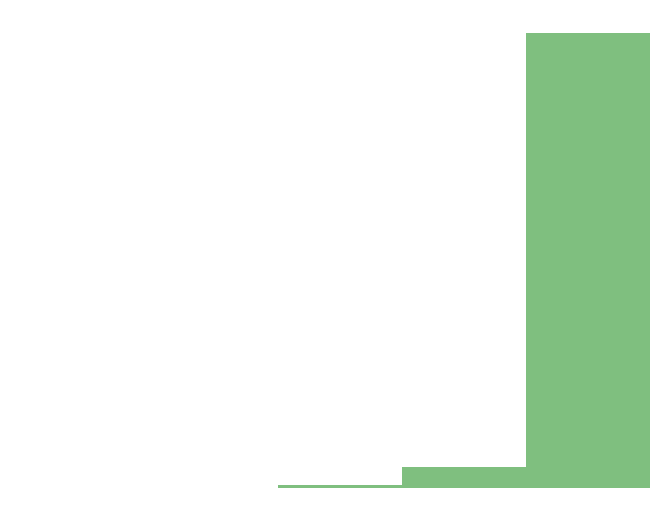
\includegraphics[width = 2cm, height = 0.5cm]{tex-inputs/data10/learnedyoursocialsecuritynumbercombined}\\
4 & video of you entering in your PIN & 92.67\% & number & 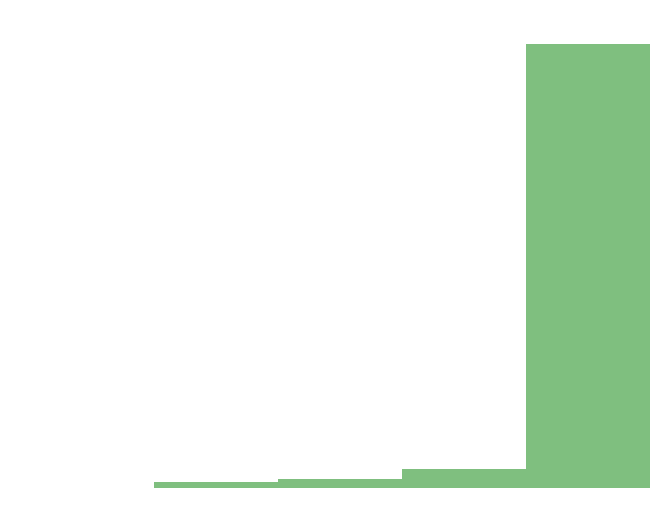
\includegraphics[width = 2cm, height = 0.5cm]{tex-inputs/data10/tookavideoofyouenteringinyourPINatanATMcombined}\\
5 & a photo of you unclothed & 92.59\% & number & \includegraphics[width = 2cm, height = 0.5cm]{tex-inputs/data10/tookaphotoofyouunclothedcombined}\\
6 & an incriminating/embarrassing photo of you & 91.39\% & number & \includegraphics[width = 2cm, height = 0.5cm]{tex-inputs/data10/tookanincriminatingphotoofyoudoingsomethingembarrassingcombined}\\
7 & username and password for websites & 89.55\% & number & \includegraphics[width = 2cm, height = 0.5cm]{tex-inputs/data10/learnedyourusernameandpasswordforwebsitescombined}\\
8 & credit card information & 88.98\% & number & \includegraphics[width = 2cm, height = 0.5cm]{tex-inputs/data10/learnedyourcreditcardinformationcombined}\\
9 & an incriminating/embarrassing video of you & 88.41\% & number & 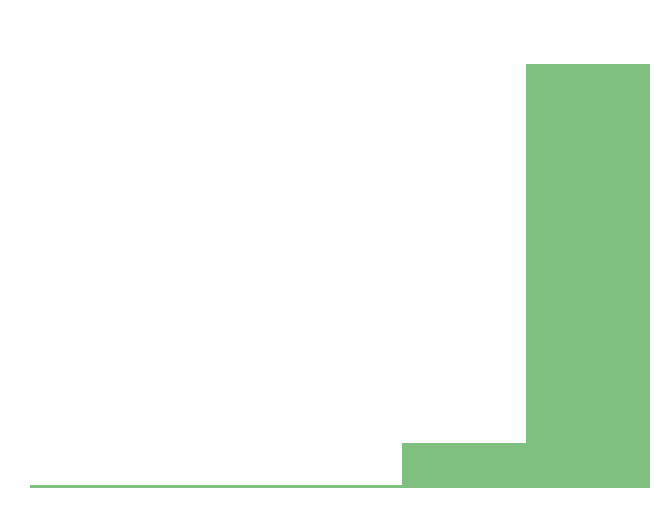
\includegraphics[width = 2cm, height = 0.5cm]{tex-inputs/data10/tookanincriminatingvideoofyoudoingsomethingembarrassingcombined}\\
10 & a random (inward-facing) photo you at home & 87.50\% & number & 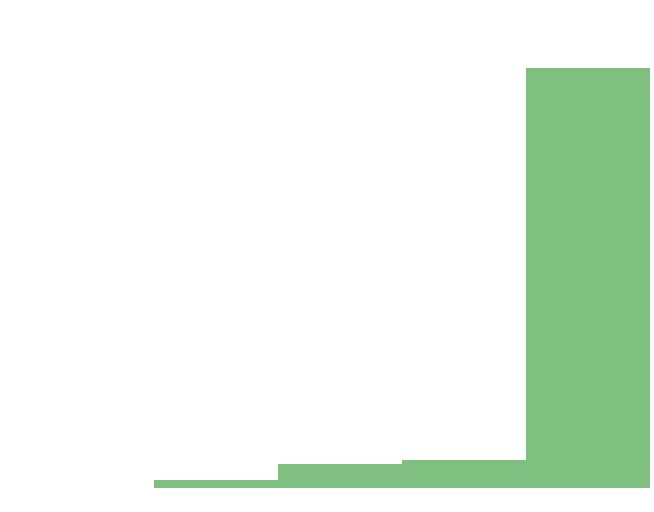
\includegraphics[width = 2cm, height = 0.5cm]{tex-inputs/data10/tookphotosofyou(withaninward-facingcamera)athomecombined}\\
 & \vdots & \\
64 & eye movement patterns (for eye tracking) & 40.51\%& number & 
\includegraphics[width = 2cm, height = 0.5cm]{tex-inputs/data10/scannedyoureyetolearnyoureyepatterns(foreyetracking)combined} \\
65 & when and how much you exercise  & 38.66\% & number & 
\includegraphics[width = 2cm, height = 0.5cm]{tex-inputs/data10/learnedwhenhowandhowmuchyouexercisecombined}\\
66 & when you are happy or having fun  & 34.75\% & number & 
\includegraphics[width = 2cm, height = 0.5cm]{tex-inputs/data10/learnedwhenyouwerehappyorhavingfuncombined}\\
67 & which television shows you watch & 30.20\% & number & 
\includegraphics[width = 2cm, height = 0.5cm]{tex-inputs/data10/learnedwhattelevisionshowsyouwatchcombined}\\
68 & when you are busy or interruptible  & 29.50\% & number & 
\includegraphics[width = 2cm, height = 0.5cm]{tex-inputs/data10/learnedwhenyouarebusyorinterruptiblecombined}\\
69 & music from your device  & 28.06\% & number & 
\includegraphics[width = 2cm, height = 0.5cm]{tex-inputs/data10/copiedanduploadedmusicfromyourdevicecombined}\\
70 & your heart rate & 27.50\% & number & 
\includegraphics[width = 2cm, height = 0.5cm]{tex-inputs/data10/learnedyourheartratecombined} \\
71 & your age & 24.29\% & number & 
\includegraphics[width = 2cm, height = 0.5cm]{tex-inputs/data10/learnedyouragecombined}\\
72 & the language you speak & 15.86\% & number & 
\includegraphics[width = 2cm, height = 0.5cm]{tex-inputs/data10/learnedthelanguageyouwerespeakingcombined}\\
73 & your gender & 15.00\% & number & 
\includegraphics[width = 2cm, height = 0.5cm]{tex-inputs/data10/learnedyourgendercombined}\\ 
\hline
\end{tabular}
\caption{The 10 most and least upsetting data types, across all recipients.}
\label{top10}
\end{center}
\end{table}



%A statistical analysis regarding the significance and confidence of <data> types with respect to all 72 was not performed due to the space constraints of the paper. We do consider all <data> categories in our statistical model, which provides an analysis of what factors had contributed to the perceived severity of a particular situation. 










%!TEX root = ../paper.tex

\subsubsection{Data Recipient}
Across all scenarios, 42.3\% of participants stated that they would be ``very upset'' if their data was shared with only the app's servers, whereas the VURs for friends (69.5\%), work contacts (75.2\%), and the public (72.4\%) were much higher. A chi-square test indicated that these differences were statistically significant (Table \ref{recipient}). However, these effect sizes were small: the largest effect was between work contacts and an app's server ($\phi=0.11$); while the VUR for sharing with work contacts was significantly higher than sharing with friends, the effect size was negligible ($\phi=0.004$). 

We note that this chi-square test violates the assumption of independent observations, since participants responded to multiple scenarios. But based on the randomization of treatments and large sample size, we do not believe that this significantly impacted our results. Similarly, we are unaware of a more appropriate test, given our data format; Cochran's Q requires binary outcomes (i.e., participants would have had to answer only one question for each data recipient, preventing us from adequately controlling for data type) and a repeated measures ANOVA requires normality (our data was not normally distributed). Nonetheless, we repeated our analysis using only one randomly-selected data point per participant and found that our selected test was robust to this violation. Participants were significantly more concerned about having their data seen by humans ({\it vis-{\`a}-vis} app servers), though differences between specific human groups (between the public, friends, and work contacts) were not significant. 

{\color {red} We do not claim that there is no distinction between the friends, public, and work contact recipients, because people have been shown to behave differently, especially in the social arena (cite studies here). People are more comfortable sharing certain data types with certain recipients (refer to the table of all questions with ranks by each recipient here). There are other data types which are universally concerning, and universally unconcerning, and the magnitude of the sentiment varies by recipient. As you can see in Table (J still needs to do this table), the VUR rate for each recipient is negatively correlated with the standard deviation of the answers.  Additionally, we see that there is greater distinction between sharing people and the app server--people are comfortable sharing data they would feel uncomfortable sharing with at human recipient, and the magnitude of concerns is might more significant compared to the other recipients.}

\begin{table}[t]
\begin{center}
\small
\begin{tabular}{| r | l | r | l |c |}
\hline
Rank & Recipient & VUR & sigma & Distribution \\
\hline
1 & Work Contacts & 75.16\% & 0.94 & 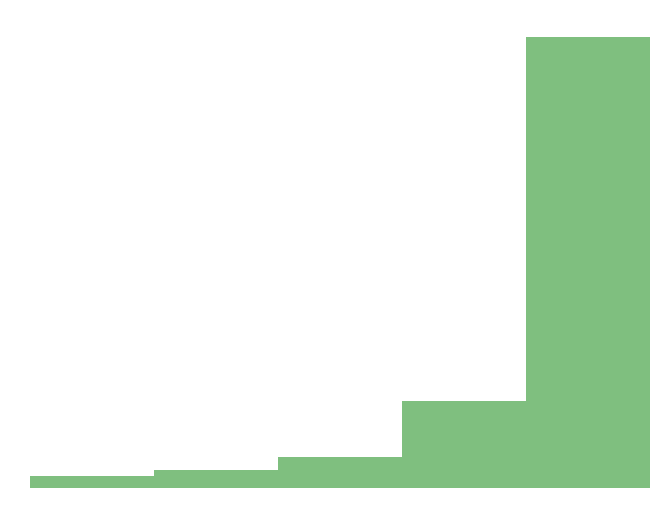
\includegraphics[width = 2cm, height = 0.5cm]{tex-inputs/recipient4/recipient_work} \\
2 & Public & 72.41\% & 0.98 & 
\includegraphics[width = 2cm, height = 0.5cm]{tex-inputs/recipient4/recipient_pub}  \\
3 & Friends & 69.47\% & 1.02 & 
\includegraphics[width = 2cm, height = 0.5cm]{tex-inputs/recipient4/recipient_friends}\\
4 & App's Server & 42.28\% & 1.15 & 
\includegraphics[width = 2cm, height = 0.5cm]{tex-inputs/recipient4/recipient_app}\\
\hline
\end{tabular}
\caption{The overall upset rate for all recipients.}
\label{recipient-table}
\end{center}
\end{table}

{\color {red} TODO: table of top and bottom 10 data types by recipient; refer to appendix; shoutout to when you were lying nervous or stressed work}

%!TEX root = ../paper.tex

\subsubsection{Data Type and Data Recipient}
%LL: This is new; It talks about the interplay between the two factors. This entire section needs work. 

We compared the 10 most concerning scenarios when sharing with an app servers versus with a humans. We observed that there was a substantial overlap between these groups, in that 6 of the most concerning scenarios were the same: \\[-.8cm]

\begin{packed_enum}
\item Bank account information
\item A video of you unclothed
\item Social security number
\item Video of you entering your PIN
\item An incriminating/embarrassing photo of you
\item A photo of you unclothed \\[-.8cm]
\end{packed_enum}

The most concerning data types do not appreciably change based on the data recipient (even the non-overlapping scenarios all dealt with confidential data such as passcodes, credit card information, etc.). However, the the level of concern range widely. For instance, the 10th most concerning scenario for the non-human audience had a VUR of 66.67\%, whereas the 10th most concerning scenario for a human audience has a VUR of 93.88\%. This suggests that the recipient determines the overall magnitude of the concern.\\

%\begin{table}[t]
%\begin{center}
%\begin{tabular}{|l|r|r|r|r|}
%\hline
%Recipients	& $\chi^2$ & p-value 	& n & $\phi$ \\
%\hline
%Work-App	& 42.49	& <0.0001	&	601	&	0.071\\
%Public-App &	48.52	& <0.0001	&		636	&	0.076\\
%Friends-App	& 32.07	& <0.0001	&		609	&	0.053\\
%Friends-Work & 	0.87 &	<0.3517	&	604	&	0.001\\
%Friends-Public	& 1.46 &	<0.2229	&	639	&	0.002\\
%Work-Public &	0.67 &	<0.7956	&		631	&	0.001\\
%\hline
%\end{tabular}
%\caption{Results of a chi-square test to examine VUR based on data recipient, across all data points.}
%\label{recipient}
%\end{center}
%\end{table}

%\begin{table}[t]
%\begin{center}
%\begin{tabular}{| c | c | c | c |}
%Recipients	& $\chi^2$ &	2-tail P &  Effect Size \\
%Work-App	& 564.318 & <0.0001 & 0.111\\
%Public-App	& 479.980 & <0.0001 &  0.092\\
%Friends-App & 380.000 & <0.0001 & 0.075\\
%Friends-Work & 20.365 & <0.0001 &  0.004\\
%Friends-Public & 5.349 & 0.0207 &  0.001\\
%Work-Public&  5.054 & 0.0246 &  0.001\\
%\end{tabular}
%\caption{Chi-Squared test results of the effects of various recipients contributing to VUR.}
%\label{recipient}
%\end{center}
%\end{table}				
%
%Commonly, bank info, SSN, PIN, embarrassing photo, naked photo, naked video were considered to be highly sensitive. When people perceived that the data would be shared with the app only, the other top five concerns included the passcode to a door, how frequently one has sex, embarrassing videos, and photos at home. When people perceived that the data would be shared with a human audience, their other top concerns were work conversations, credit card information, username and password combinations for websites, and phone conversations. When data is perceived to be shared by an app, people are more concerned with issues of being spied on or tracked, whereas when data is perceived to be shared with an individual, people are concerned more with theft or reputation. 
%
%On the other hand, exercise details, age, tv shows, gender, heart rate, and language were commonly considered to be lease concerning. When people perceived that the data would be shared with the app only, the other indifferent data included phone use, how much one liked the people around, when and what you ate, and eye patterns. When people perceived that the data would be shared with a human audience, the least concerning data included one's name, if one was having fun, music on the device, and if one was busy or interruptible. When sharing with an application, information otherwise considered personal such as phone use, opinions of people, food eaten, or eye patterns were okay to share, since these seem like useful information to improve one's device experience. However, people are not likely to share the same with people, but are more comfortable with sharing data about topics which would come up in causal conversation.
%!TEX root = ../paper.tex


\begin{table}[t]
\begin{center}
\begin{tabular}{| c | r | r |}
\hline
 Misbehavior &  Cubetastic3000 & Smartphone \\
 \hline
 \hline
 All & 58.79\% & 46.67\%\\
 \hline
Vibration & 14.81\%  &  6.14\%\\
Bluetooth & 44.12\%  &  19.86\%\\
Unmuted Call & 87.10\%  &  58.44\%\\
Screenshot & 52.78\%  & 55.74\%\\
Premium Calls/Texts & 86.49\%  &  91.94\%\\ 
\hline
\end{tabular}
\caption{VURs for the five questions about device misbehaviors described in Section \ref{sec:smartphones}, contrasting smartphones with the Cubetastic3000.}
\label{deviceVUR}
\end{center}
\end{table}

\subsubsection{Device}
Recall that each participant answered 2 questions drawn from a set of 5 regarding their reactions to smartphone misbehaviors. To compare these misbehaviors with misbehaviors on the Cubetastic3000, we included these same 5 questions amongst the pool of 293 Cubetastic3000 scenarios, only modifying the device type. In this manner, while all 1,782 participants received 2 smartphone questions, there were 159 participants who received at least one of these questions in relation to the Cubetastic 3000. Across all participants, the VUR was 46.7\% (of 1,782) when describing smartphones, whereas the VUR increased to 58.8\% (of 159) when describing these same misbehaviors on the Cubetastic3000. The VURs for both devices for all 5 questions are in Table ~\ref{deviceVUR}.

To preserve data independence, we performed a Mann-Whitney U test by comparing participants' average VURs for the Cuebtastic3000 scenarios (i.e., 159 participants) to the remaining participants' average VURs for the smartphone scenarios (i.e., 1,623 participants). We found this difference to be statistically significant ($108,664.0$, $p<0.0005$), however, the effect size was incredibly small ($r=0.08$). Because of this small effect size, we did not further reduce our statistical power by separately comparing each of the 5 misbehaviors. As a result, we can conclude that in general users are likely to be more wary of misbehaviors occurring on wearable devices than smartphones, the difference is likely negligible. Similarly, the entire effect may be due to participants' increased familiarity with smartphones, and therefore may disappear as they increasingly encounter more wearable devices.

%{\color {red} talk about the variance of the devices in general--was there more spread for the answers wrt smartphones, cubetastic, or were they kind of all the same?}



						
%\begin{table}%[h]
%\begin{center}
%\begin{tabular}{| c | c | c | c |}
%Question & $\chi^2$ &	2-tail P & Effect Size \\
%All & 0.444  & 0.505 & 0.006\\
%Q1 & 0 & 1 & 0 \\
%Q2 & 0 & 1 & 0\\
%Q3 & 0 & 1 & 0\\
%Q4 & 0 & 1 & 0\\
%Q5 & 0 & 1 & 0\\
%\end{tabular}
%\caption{Results of the effects of <device> type contributing to VUR. Values are McNeamar's test results for within-subjects comparisons for participants who received both questions.}
%\label{withindevice}
%\end{center}
%\end{table}

%For the between-subjects comparison (i.e., participants who received one question, but not the other), you can do either a chi-square test or Fisher's exact test. Both use a 2 x 2 contingency matrix (i.e., rows are outcomes---upset or not---and columns are conditions---wearable or smartphone). The way to choose between the two tests is based on sample size, generally you use chi-square when there are more than 10-20 samples per cell in the table, but using either is just as valid. For the within-subjects comparisons (i.e., participants received both questions), you would do McNemar's test; which is the within-subjects version of the chi-square test. 

%!TEX root = ../paper.tex
\subsubsection{Demographic Factors}

Participants' responses were correlated with demographic factors. We observed that the biggest predictor of participants' decisions to rate a scenario as very upsetting was their self-reported level of general privacy concerns, as determined by the IUIPC scale~\cite{malhotra2004internet}. A Spearman correlation yielded a statistically significant effect between average IUIPC scores with the VUR ($\rho=0.446$, $p<0.0005$), which suggests that people's responses to questions were mostly based on their privacy preferences. Additionally, we observed that age was a significant predictor of VUR ($\rho=0.121$, $p<0.0005$). We suspect that the effect of age is due to the significant correlation between age and IUIPC scores ($\rho=0.188$, $p<0.0005$); others have observed that older individuals tend to be more protective of their privacy~\cite{varian2005demographics}.

While we initially observed an effect on VURs based on whether or not participants claimed to already own wearable devices (57.0\% vs. 60.8\%, respectively; Mann-Whitney $U=202,896$, $p<0.032$), this difference did not remain significant upon correcting for multiple testing (Bonferroni corrected $\alpha=0.01$). The effect of a participant's gender also did not remain significant upon correcting for multiple testing. We observed no correlation between a participant's education level and VUR.
%!TEX root = ../paper.tex

\subsubsection{Regression Models} 
\label{sec:regression}
In order to examine the relative effect of each factor on participants' VURs, we construct several statistical models to predict whether a participant would be ``very upset'' with a given scenario based on the data type, data recipient, and their demographic factors (i.e., age, education, gender, and privacy attitudes). We perform binary logistic regressions using generalized estimating equations, which account for our repeated measures experimental design (i.e., each participant contributed multiple data points).

\begin{table}[t]
\centering
\begin{tabular}{|l| r| r| r|}
\hline
Parameters & $\chi^2$ & $df$ & QIC\\
\hline
\hline
(Intercept) & 423.96 & 1 & 13,209.1\\
\hline
(Intercept) & 207.07 & 1 & 12,551.49\\
IUIPC (covariate) & 368.5 & 1 & \\
Gender (covariate) & 6.30 & 1 & \\
\hline
(Intercept) & 411.66 & 1 &12,458.86\\
Data Recipient & 599.72 & 3 & \\
\hline
(Intercept) & 418.02 & 1 & 11,382.75\\
Data Type & 1,141.40 & 71 & \\
\hline
(Intercept) & 66.18 & 1 & 9,609.65 \\
Data Recipient & 617.25 & 3 & \\
Data Type & 1,288.51 & 71 & \\
IUIPC (covariate) & 105.73 & 1 & \\
Gender (covariate) & 9.74 & 1 & \\
IUIPC $\times$ Gender & 8.33 & 1 &\\
\hline
\end{tabular}
\caption{Goodness-of-fit metrics for various binary logistic models of our data using general estimating equations to account for repeated measures. The columns represent the Wald test statistic for each parameter and the overall Quasi-Akaike Information Criterion (QIC) for each model. Each parameter listed was statistically significant at $p<0.005$.}
\label{regression}
\end{table}

We create several models using two independent variables as predictors: data and recipient. Because the device (i.e., whether they were using the Cubetastic3000 or a smartphone) is only varied for the five smartphone misbehaviors listed in Section \ref{sec:smartphones}, we removed these five  from our models, which resulted in a total of 72 types of data shared with 4 possible recipients. We also used collected demographic factors as covariates: age, gender, education, wearable device ownership (yes/no), and mean IUIPC score. For each model, we performed Wald's test to examine the model effects attributable to each of these parameters. The only covariates that had an observable effect on our models were gender and participants' IUIPC scores, which also exhibited an interaction effect with each other. Thus, we opted to remove the other covariates from our analysis. Table \ref{regression} shows the various models that we examined and the Quasi-Akaike Information Criterion (QIC), which is a goodness-of-fit metric for model selection that also accounts for complexity (lower relative values indicate better fit). As can be seen, the data type was the strongest predictor of VUR.

While these models illustrate the relative weights that users place on information when determining a scenario as truly upsetting, one shortcoming of this approach is its generalizability: the data predictor is categorical and limited to the data that we specifically chose for this study. To make our data set more generalizable to other use cases, we coded each data type in two ways: in terms of broad descriptions of the type of data (e.g., video, audio, etc.) and the type of risk it presents. Two researchers agreed on a codebook and independently coded each of the 72 data types.

The data types fell into the following six possible categories:
\begin{enumerate}[topsep=0pt,itemsep=-1ex,partopsep=1ex,parsep=1ex]
\item Photo
\item Video
\item Audio
\item Behavioral Information
\item Biometric Information
\item Demographic Information
\end{enumerate}

While the first three categories are self-explanatory, the latter three categories are all based on different user characteristics. We defined {\it behavioral information} as observations about the user's activities; {\it biometric information} as measurements of the user's body; and {\it demographic information} as non-biometric information about the user's traits. 

The risks for each data type fell into the following categories:
\begin{enumerate}[topsep=0pt,itemsep=-1ex,partopsep=1ex,parsep=1ex]
\item {\bf Financial:} the loss of money or property.
\item {\bf Image:} the loss of control over one's self-image (e.g., publicizing something embarrassing).
\item {\bf Medical:} the disclosure of medical information.
\item {\bf Physical:} physical harm to the user.
\item {\bf Relationships:} damage to the user's inter-personal relationships.
\end{enumerate}

After independently coding, the researchers met to resolve any disagreements, such that the results reflect unanimity. There was  83\% agreement prior to resolution. Cohen's $\kappa$ was 0.81 for the data categories and 0.75 for the  risk categories, both indicating ``excellent'' agreement~\cite{Fleiss2003}. 

With regard to data types, the most concerning type of data is video (78.0\%), which was ranked similarly to photos (76.2\%). Next are audio (66.8\%) and demographic data (65.4\%), followed by behavioral (53.1\%) and biometric (46.3\%) data. We suspect that demographic data was more concerning because it included information such as a Social Security Number, bank account information, and other financial information. We chose to categorize them as such as they are non-biological descriptors of the user. We were very surprised that biometric information was seen as relatively benign compared to the other broad categories of data. One hypothesis is that since most home users do not use biometric authentication, they may have an inaccurate understanding of the types of systems that might be at risk if biometric data is stolen and abused.

With regard to the presented risks, we observed that average VURs were highest for financial information disclosure (82.0\%). Information regarding relationships (69.2\%), physical safety (66.4\%), and self-image (65.8\%) followed. VURs were lowest for medical information disclosure (47.4\%). One reason why medical risks were ranked relatively low is that this category broadly covered scenarios involving data about the user's health, but also included more basic medical information, such as age, gender, and emotional state. As mentioned in Section \ref{sec:datatypes}, participants saw these as publicly observable and unconcerning.


\begin{table}[t]
\centering
\begin{tabular}{|l| r| r| r|}
\hline
Parameters & $\chi^2$ & $df$ & QIC\\
\hline
\hline
(Intercept) & 442.66 & 1 & 12,727.42\\
Risk & 405.18 & 4 & \\
\hline
(Intercept) & 380.39 & 1 & 12,681.86\\
Data Category & 439.45 & 5 & \\
\hline
(Intercept) & 256.15 & 1 & 12,061.87\\
Risk & 157.84 & 4 & \\
Data Category & 183.90 & 5 & \\
Risk $\times$ Data Category & 259.81 & 8 & \\
\hline
(Intercept) & 62.65 & 1 & 10,406.35\\
Risk & 205.21 & 4 & \\
Data Category & 250.35 & 5 & \\
Recipient & 546.89 & 3 & \\
IUIPC (covariate) & 103.94 & 1 & \\
Gender (covariate) & 9.80 & 1 & \\
IUIPC $\times$ Gender & 8.21 & 1 & \\
Risk $\times$ Data Category & 303.44 & 8 & \\
Recipient $\times$ Risk & 39.14 & 12 & \\
\hline
\end{tabular}
\caption{Metrics for additional binary logistic models of our data using general estimating equations to account for repeated measures. The columns represent the Wald test statistic for each parameter and the overall Quasi-Akaike Information Criterion (QIC) for each model. Each parameter listed was statistically significant at $p<0.005$.}
\label{regression2}
\end{table}


Using these two new variables as additional independent variables (and removing the previous data type variable), we created a second set of models. Because these risk categories and mediums are less likely to change over time, models that take these into account are likely to be more useful and less likely to be overfit. What these models show us is that both risk and medium are relatively strong predictors by themselves, and have an even stronger interaction effect. When the data recipient and covariates are added to the model, the resulting goodness-of-fit is not much worse than that of the model using the actual data type. %The full model can be found in Appendix \ref{sec:regression-apx2}.


%!TEX root = ../paper.tex

\subsection{Risk and Benefit Rankings} 
\begin{figure}[t]
	\centering
	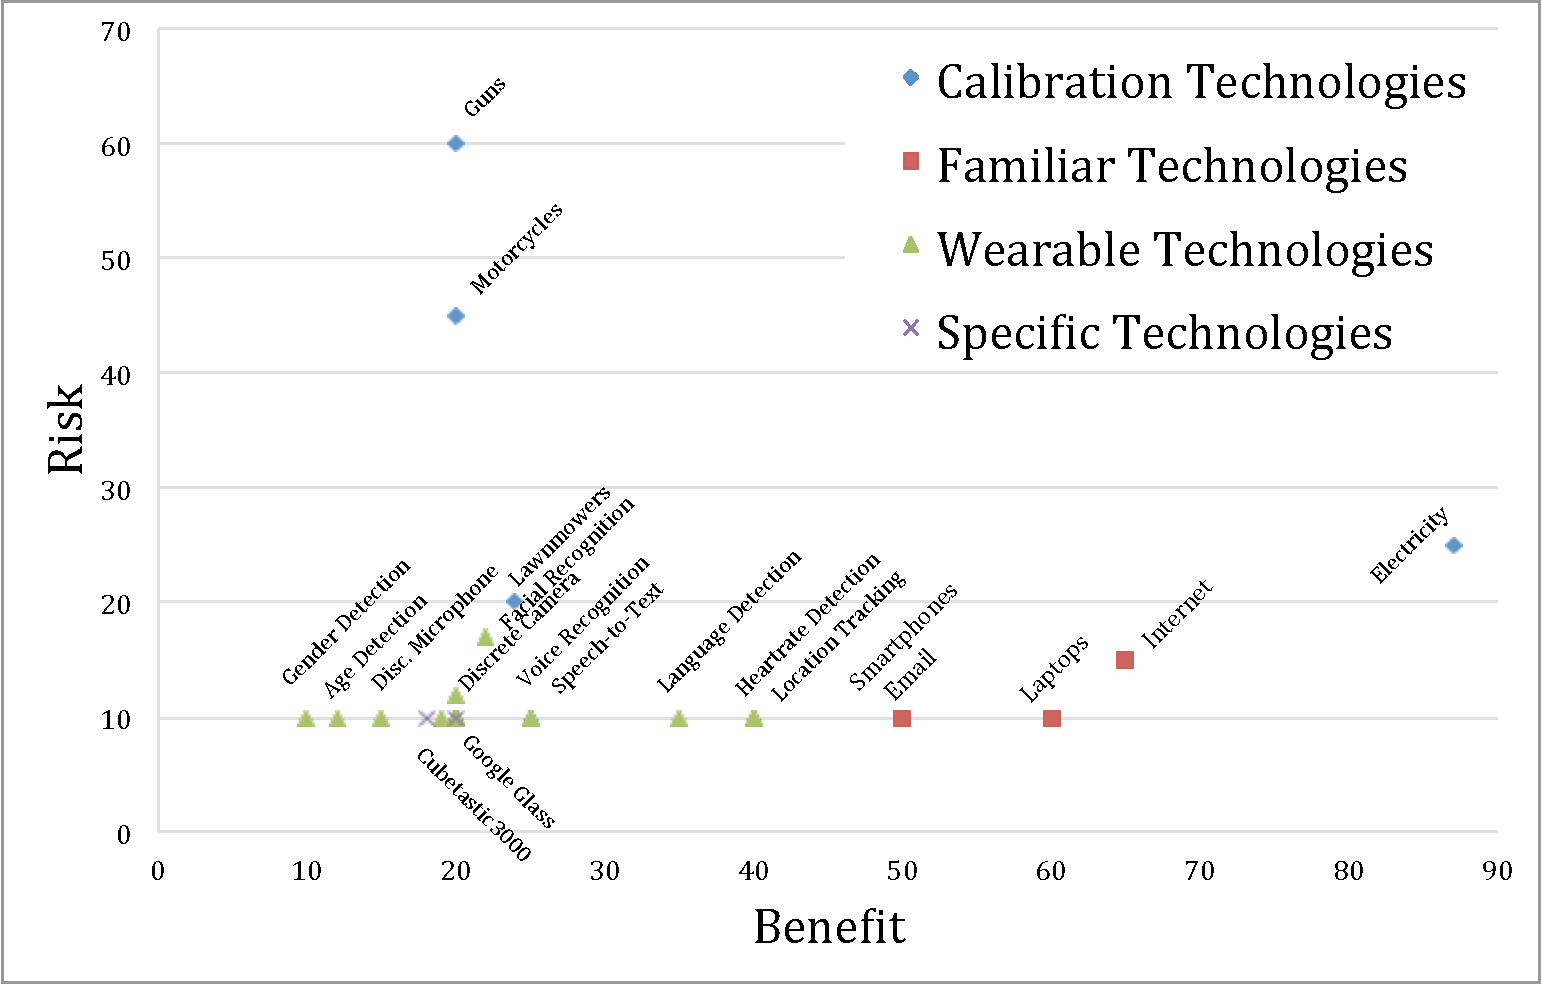
\includegraphics[width=\columnwidth]{images/riskbenefit.pdf}
	\caption{Participants' median risk-benefit ratings of technologies examined by Fischhoff \etal\cite{Fischhoff}, which we used for calibration, alongside familiar technologies (e.g., laptops, the Internet, etc.), wearable technologies, as well as two specific wearable devices (Google Glass and the Cubetastic3000).}
	\label{fig:techplot}
\end{figure}

We asked participants to rate new capabilities related to wearable technologies (e.g., facial recognition) in terms of their risks and benefits. We also asked them to do this for technologies with which they were likely to be more familiar (e.g., smartphones and laptops) in addition to two examples of specific wearable devices, Google Glass and the fictitious Cubetastic3000. To calibrate our results, we also asked about four well-established technologies studied by Fischhoff \etal\cite{Fischhoff}. We found that participants generally rated technologies related to wearables as being low-risk comparatively to other technologies (Figure \ref{fig:techplot}). Tables \ref{risk} and \ref{benefit} in Appendix ~\ref{sec:concerns-appendix} shows participants' median, quartiles, and distributions of risks and benefit ratings for all technologies. We found that the calibration technologies, which were more familiar to the participants, were all rated as the most risky. 

As a group, participants rated more familiar technologies as more beneficial. We believe this is the result of exposure to these technologies---most people use these technologies daily and therefore see what the benefits of these technologies are. It is true that people perceive unfamiliar technologies as less beneficial at the moment, but this will change as the use of these technologies evolve and adoption increases. Most calibration technologies, with the exception of electricity, were seen as lower benefit than the others. However, Google glass and Cubetastic3000 were about equally beneficial, and gender and age recognition were less beneficial. 

Of the wearable technologies, the riskiest technologies included facial recognition, the Internet, and discrete cameras, whereas the remainder of the technologies were seen as having minimal, equivalent risk levels (i.e., a median of ``10''). We did not test the differences in risk between the different wearable-related technologies for statistical significance, but given their minimal spread compared to the calibration options, the differences appears to be negligible. Interestingly, privacy risks were perceived as being comparable to physical risks; for instance, the capacity for facial detection on a wearable device was perceived as being almost as risky as interacting with a lawnmower. 

Participants were prompted to rate technologies with respect to all considerations (see Appendix~\ref{sec:prompt}), including risk of physical harm to bystanders, financial cost, distress, misuse, or impact on public, personal, and private life. Participants may have still evaluated the risks with an emphasis toward physical risk and without an emphasis on privacy risk. Among the five presented options, the wearable-related one is the only one without some physical risk scenario, and physical risk is a clear, tangible risk. 

We examined participants' perceptions, and therefore responses may not be reflective of actual risks or benefits. However, they also reflect the general public's exposure to these technologies and show that people perceive specific risks and benefits. We suspect that the similarity in assessments between the various wearable technologies are because most people are not consciously aware of the possibilities and that performing this experiment longitudinally may yield more interesting results, as these technologies become pervasive (and more familiar to participants).

%!TEX root = ../paper.tex
\subsection{Open-Ended Concerns for Wearables}
We captured participants' reactions to wearable devices as a whole by asking the following open-ended question:

\begin{quotation}
\noindent
\textit{What do you think are the most likely risks associated with wearable devices?}
\end{quotation}

This question was asked with demographics questions, but before any IUIPC questions (which asked a lot of direct privacy-related questions, to avoid biasing the recipients). The participants were presented with a blank box to write in, with no character limit to their open-ended responses. 

Table \ref{openresponses} shows common user concerns related to wearable devices. Appendix \ref{sec:coding} details the responses categorized in each coding label. Most are related to privacy and security, but this open-ended data gives a sense of what broad categories of concerns are most relevant to users. This can be used to guide research in unexplored use cases. 

In addition to privacy and security in the general sense, significant concerns included being unaware of what the device is collecting, doing, or which information it is using (Being Unaware). Other orthogonal concerns included long-term health effects caused from wearing the device such as cancer from EMF waves (Health) and safety hazards from wearing the device, such as distractions that cause car accidents (Safety). Interestingly, participants were also concerned with resulting changes in social behaviors, such as dependence on devices or spending less time with loved ones (Social Impact). 

\begin{table}[t]
\begin{center}
\begin{tabular}{|l|r|r|}
\hline
Concern &  Responses &  Frequency   \\
\hline
Privacy & 452 & 25.32\% \\
Being Unaware & 275 & 15.40\% \\
%Unaware Use & 167 & (9.36\%)\\
%Unaware Collection & 64 & (3.59\%)\\
%Unaware Access & 44 & (2.46\%)\\
Health Risk & 191 & 10.70\%\\
Safety & 185 & 10.42\%\\
Social Impact &	157 & 8.80\%\\
Financial Cost & 151 & 8.46\%\\
Security &	144 & 8.07\%\\
Accidental Sharing &	69 & 3.87\%\\
Miscellaneous &	57 & 3.19\%\\
None	& 51 & 2.86\%\\
Social Stigma &	39 & 2.18\%\\
False Information & 33 & 1.85\%\\
Don't know & 31 & 1.74\%\\
Aesthetics 	& 19 & 1.06\%\\
Don't care 	& 11 & 0.62\%\\
\hline
\end{tabular}
\caption{The most common open-ended risks associated with owning a wearable device.}
\label{openresponses}
\end{center}
\end{table}

%!TEX root = ../paper.tex

\section{Discussion}
%We discuss considerations when interpreting our results, the limitations of our work, and future work we hope to inspire. 

%\subsection{Limitations}
One of the limitations is that our participants might not have interest in or knowledge of wearables and their respective capabilities, since 83\% of our participants reported that they do not own a wearable. Participants may be over or underestimating the risk due to unawareness of what can be inferred from the data, not have an idea of how to rate a new technology with respect to familiar ones, or be more influenced by recent events.\footnote{Recently, stories of exploding batteries were in the news~\cite{1_levin_2014}, which were explicitly reported as a concern in our open-ended question.}  For instance, biometrics were generally not a concern for our participants, although there are many security and privacy implications~\cite{prabhakar2003biometric}.

We recruited both wearable users and non-users in order to yield a more representative sample of the general population. We could have easily recruited only wearables owners or people specifically interested in wearables. However, that would have its own biases and limitations. At the time of this writing, about 85\% of the general population do not own wearable devices~\cite{Nilsen,WearableStatNews}, indicating our study is reflective of the current population. 

Because of the privacy paradox, participants' stated responses may differ from how they may react to these same scenarios in real life~\cite{norberg2007privacy, jensen2005privacy}. At the same time, our results do reflect actual perceptions of wearable devices and the associated privacy scenarios involving them. This is an unavoidable, yet important distinction to make with of studies of this nature: our primary goal was to examine perceptions and preferences, so that future systems can be designed with these in mind. We do not expect that such systems will satisfy users in all situations, however, we believe that user-centered design will still be a vast improvement over post hoc approaches (or ignoring user concerns altogether).

%\subsection{Future Research Directions}
Further work can be done to expand various aspects of this study. Investigating more fine-grained data types (e.g., investigating specific instances of location data, versus location data in general) would be a useful endeavor to gain further insight into user perceptions. Adding additional recipients, such as ``advertisers'' or ``acquaintances'' may lead to more nuanced results. Additionally, the open-ended concerns illuminate areas of possible future research, such as communication and minimization of health effects from use, designing distraction-free interfaces to prevent safety issues, and minimizing negative social impacts during use.  
%!TEX root = ../paper.tex

\section{Related Work}
%%% better introduction, or take this out. This seems awkward. 
%We discuss related work that has examined users' perceptions surrounding security and privacy risks.

\subsection{Ubiquity and Wearable Devices}
Many authors have emphasized that we are rapidly moving towards a world of ubiquitous sensing and data capture, with ensuing privacy challenges~\cite{abowd2000charting,palen2003unpacking,camp2000internet}. Many researchers have worked to study how privacy can be preserved in the presence ubiquitous devices. Examples of such efforts include frameworks to design for privacy~\cite{bellotti1993design,camp2003designing,langheinrich2001privacy}, protocols for anonymous communication {cornelius2008anonysense}, evaluation metrics for privacy ~\cite{scholtz2004toward}, and privacy models ~\cite{hong2004privacy, jiang2002approximate}. However, none of these works attempted to quantify or rank user concern over different privacy risks. 

Roesner et al.\ urge the community to address potential concerns for wearable devices before the technologies become widespread \cite{roesner2014security} and explore the unique and difficult problems these devices present in terms for law and policy \cite.{roesner2014augmented}. A small-scale interview of how bystanders feel about wearable devices found that bystanders were predominantly split between having indifferent and negative reactions to the device but expressed clear interest in being able to give permissions for the data being captured \cite{denning2014situ}. We hope our research furthers   work in communicating with users and bystanders. 

\subsection{Smartphones}
Many researchers have attempted to study user concerns about security or privacy issues associated with their smartphones. Research shows that perceptions of risk change as computing systems change. Chin et. al\ investigate how user attitudes toward security and privacy for smarphones differ from attitudes for traditional computing systems, and find that these attitudes differ significantly ~\cite{chin2012measuring}. How people use these devices had also changed. Palen et. al\ track smartphone users for six weeks to find rapid modifications in behaviors with respect to context and the social appropriateness of phone use cite\{palen2000going}. People also perceive and behave without a realistic understanding of the risks they are taking. Felt et. al\ examine the Android permission system and find that 17\% of participants paid attention to permissions, and only 3\% comprehended what these permissions meant.  

%%% There's way more work in this area that needs to be cited (look at stuff by Janne Lindqvist, Norman Sadeh, Patrick Kelley, and Jason Hong). At the very least, if you don't add new citations, you absolutely need to say 2-3 sentences about the three papers that you did cite. Though I strongly urge you to add more.

\subsection{User Perceptions and Behaviors}
In this paper we focus on measuring people's perceptions of security and privacy risks. One limitation of user perceptions is that people don't always have enough information to make privacy-sensitive decisions; even if they do, they often trade off long-term privacy for short-term benefits~\cite{acquisti2005privacy}. Also, actual behavior may deviate from self-reported behaviors~\cite{jensen2005privacy} and privacy preferences~\cite{spiekermann2001privacy}.

While risk communication for the physical world has been examined for several decades (e.g.,~\cite{Fischhoff,Morgan2001}), research into effectively communicating computer-based risks has only recently been researched. For example, both Garg et al.\ and Blythe et al.\ show that due to varying perceptions and abilities that correlate with demographic factors, computer-based risk communication should employ some degree of demographic targeting~\cite{Garg2012,Blythe2011}. While this work is likely applicable to wearable computing risk communication, we believe that a better understanding of users' risk perceptions in this domain is warranted prior to examining risk communication. 
%!TEX root = ../paper.tex

\section{Conclusion}

 Our survey of 1,784 Internet users, is the first large-scale study to investigate user-centric security and privacy concerns for wearable devices. We contribute a comprehensive ranking of possible risks associated with wearable devices, across various recipients. We calibrate our results with mobile devices and existing technologies; additionally, we verify with an open-ended question and find that privacy and security are at the top of user's overall concerns. Wearables are still in their infancy. Perceptions of situations and capabilities will change rapidly with advancements and increased exposure. However, there is not much work done to determine which threats in the emerging threat landscape are pertinent to focus on. Inspection of possible data concerns agree with previous studies of smartphone studies to find that video capture and financial data to be most sensitive. Various systems which detect and take actions for sensitive objects in photos and videos will be critical as wearables and other devices become more ubiquitous. We also find that users' self-reported privacy preferences are correlated with how participants may react, even with respect to situations that they are unfamiliar with. Permissions and access control mechanisms which do not depend on user inputs can still benefit from being informed by user preferences. We hope that this work has given a comprehensive overview of user concerns and inform designs of future privacy and security work for wearable devices.  

%\begin{table}{| p{0.5cm} | p{7cm} | p{1cm} | c |}

\hline \multicolumn{1}{|c|}{\textbf{Rank}} & \multicolumn{1}{c|}{\textbf{Question}} & \multicolumn{1}{c|}{\textbf{VUR(\%)}} &  \multicolumn{1}{c|}{\textbf{Distribution}} \\ \hline 
\endfirsthead

\multicolumn{3}{c}%
{{\bfseries \tablename\ \thetable{} -- continued from previous page}} \\
\hline \multicolumn{1}{|c|}{\textbf{Rank}} & \multicolumn{1}{c|}{\textbf{Question}} & \multicolumn{1}{c|}{\textbf{VUR(\%)}} &  \multicolumn{1}{c|}{\textbf{Distribution}} \\ \hline 
\endhead

\hline \multicolumn{4}{|r|}{{Continued on next page}} \\ \hline
\endfoot
\hline 
\endlastfoot
1 & Tookavideoofyouunclothed & 95.97 & \includegraphics[width = 2cm, height = 0.5cm]{tookavideoofyouunclothedcombined} \\ 
2 & Learnedyourbankaccountinformation & 95.91 & 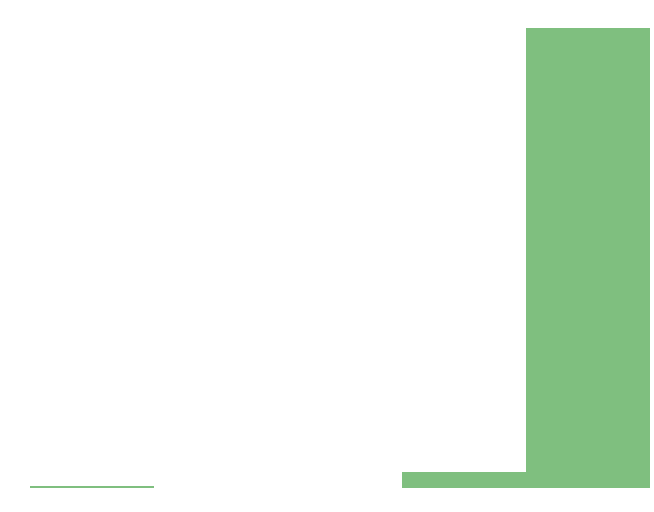
\includegraphics[width = 2cm, height = 0.5cm]{learnedyourbankaccountinformationcombined} \\ 
3 & Learnedyoursocialsecuritynumber & 94.84 & 
\includegraphics[width = 2cm, height = 0.5cm]{learnedyoursocialsecuritynumbercombined} \\ 
4 & Tookavideoofyouenteringinyourpinatanatm & 92.67 & 
\includegraphics[width = 2cm, height = 0.5cm]{tookavideoofyouenteringinyourPINatanATMcombined} \\ 
5 & Tookaphotoofyouunclothed & 92.59 & \includegraphics[width = 2cm, height = 0.5cm]{tookaphotoofyouunclothedcombined} \\ 
6 & Tookanincriminatingphotoofyoudoingsomethingembarrassing & 91.39 & \includegraphics[width = 2cm, height = 0.5cm]{tookanincriminatingphotoofyoudoingsomethingembarrassingcombined} \\ 
7 & Learnedyourusernameandpasswordforwebsites & 89.55 & \includegraphics[width = 2cm, height = 0.5cm]{learnedyourusernameandpasswordforwebsitescombined} \\ 
8 & Learnedyourcreditcardinformation & 88.98 & \includegraphics[width = 2cm, height = 0.5cm]{learnedyourcreditcardinformationcombined} \\ 
9 & Tookanincriminatingvideoofyoudoingsomethingembarrassing & 88.41 & 
\includegraphics[width = 2cm, height = 0.5cm]{tookanincriminatingvideoofyoudoingsomethingembarrassingcombined} \\ 
10 & Tookphotosofyou(Withaninward-Facingcamera)Athome & 87.5 & 
\includegraphics[width = 2cm, height = 0.5cm]{tookphotosofyou(withaninward-facingcamera)athomecombined} \\ 
 & \vdots & & \\
64 & Scannedyoureyetolearnyoureyepatterns(Foreyetracking) & 40.51 & 
\includegraphics[width = 2cm, height = 0.5cm]{scannedyoureyetolearnyoureyepatterns(foreyetracking)combined} \\ 
65 & Learnedwhenhowandhowmuchyouexercise & 38.66 & 
\includegraphics[width = 2cm, height = 0.5cm]{learnedwhenhowandhowmuchyouexercisecombined} \\ 
66 & Learnedwhenyouwerehappyorhavingfun & 34.75 & 
\includegraphics[width = 2cm, height = 0.5cm]{learnedwhenyouwerehappyorhavingfuncombined} \\ 
67 & Learnedwhattelevisionshowsyouwatch & 30.2 & 
\includegraphics[width = 2cm, height = 0.5cm]{learnedwhattelevisionshowsyouwatchcombined} \\ 
68 & Learnedwhenyouarebusyorinterruptible & 29.5 & 
\includegraphics[width = 2cm, height = 0.5cm]{learnedwhenyouarebusyorinterruptiblecombined} \\ 
69 & Copiedanduploadedmusicfromyourdevice & 28.06 & 
\includegraphics[width = 2cm, height = 0.5cm]{copiedanduploadedmusicfromyourdevicecombined} \\ 
70 & Learnedyourheartrate & 27.5 & 
\includegraphics[width = 2cm, height = 0.5cm]{learnedyourheartratecombined} \\ 
71 & Learnedyourage & 24.29 & 
\includegraphics[width = 2cm, height = 0.5cm]{learnedyouragecombined} \\ 
72 & Learnedthelanguageyouwerespeaking & 15.86 & 
\includegraphics[width = 2cm, height = 0.5cm]{learnedthelanguageyouwerespeakingcombined} \\ 
73 & Learnedyourgender & 15.0 & 
\includegraphics[width = 2cm, height = 0.5cm]{learnedyourgendercombined} \\ 
\end{stable}

\end{document}
%\input{ranks.tex}
\begin{table}[H!]
\begin{center}
\small
\begin{tabular}{| p{2cm} | p{1cm} | p{1cm} | p{1cm} | c |}
\hline
Technology & Q1 &  Median & Q3 & Distribution  \\ 
\hline
Voice Based Emotion Detection  & 10.0 & 10.0 & 15.0 & 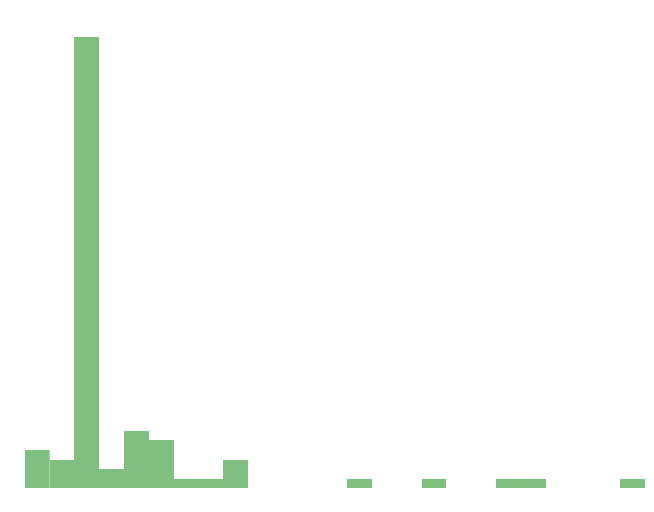
\includegraphics[width = 2cm, height = 0.5cm]{tables/voicebasedemotiondetectionrisk} \\ 
Facial Detection  & 10.0 & 10.0 & 25.0 & 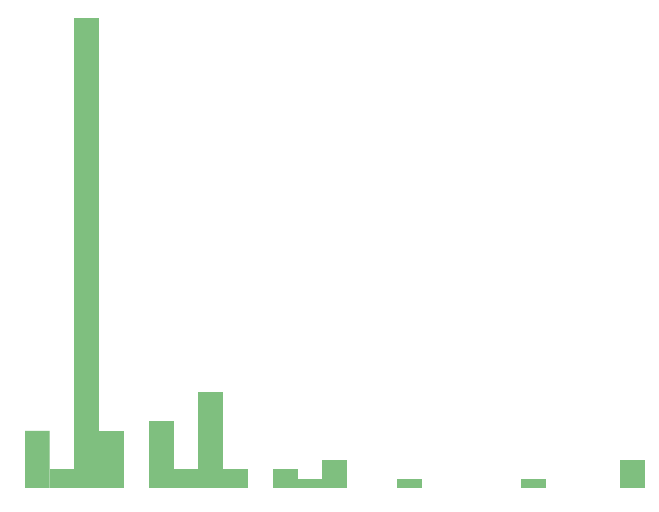
\includegraphics[width = 2cm, height = 0.5cm]{tables/facialdetectionrisk} \\ 
Facial Recognition  & 10.0 & 17.0 & 30.0 & 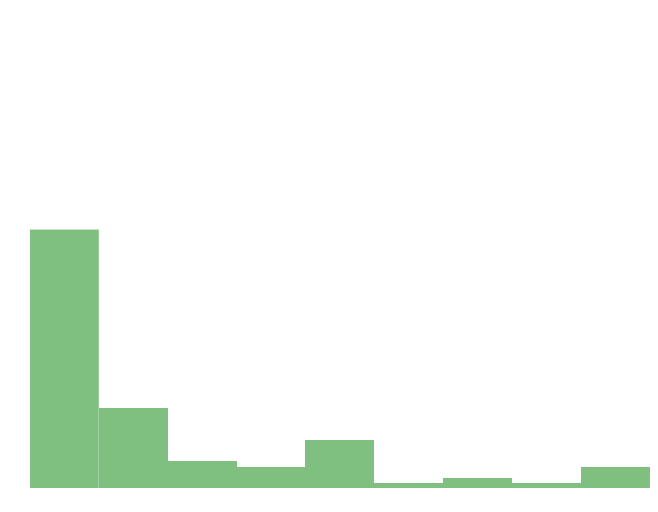
\includegraphics[width = 2cm, height = 0.5cm]{tables/facialrecognitionrisk} \\ 
Language Detection  & 10.0 & 10.0 & 10.0 & 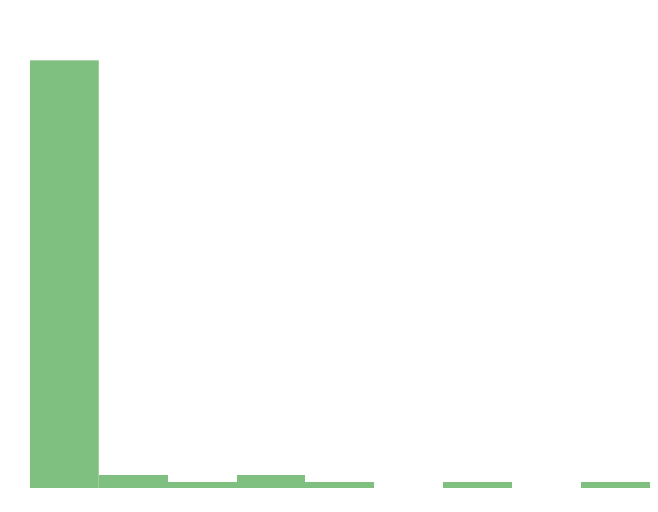
\includegraphics[width = 2cm, height = 0.5cm]{tables/languagedetectionrisk} \\ 
Gender Detection  & 10.0 & 10.0 & 13.5 & \includegraphics[width = 2cm, height = 0.5cm]{tables/genderdetectionrisk} \\ 
Heart Rate Detection  & 10.0 & 10.0 & 10.0 & \includegraphics[width = 2cm, height = 0.5cm]{tables/heartratedetectionrisk} \\ 
Age Detection  & 10.0 & 10.0 & 15.0 & \includegraphics[width = 2cm, height = 0.5cm]{tables/agedetectionrisk} \\ 
Smartwatches  & 10.0 & 10.0 & 10.0 & \includegraphics[width = 2cm, height = 0.5cm]{tables/smartwatchesrisk} \\ 
Discreet Microphone  & 10.0 & 10.0 & 20.0 & \includegraphics[width = 2cm, height = 0.5cm]{tables/discreetmicrophonerisk} \\ 
Location Tracking  & 10.0 & 10.0 & 20.0 & \includegraphics[width = 2cm, height = 0.5cm]{tables/locationtrackingrisk} \\ 
Electricity & 15.0 & 25.0 & 40.0 & \includegraphics[width = 2cm, height = 0.5cm]{tables/ElectricityRisk} \\ 
Speech To Text  & 10.0 & 10.0 & 10.0 & \includegraphics[width = 2cm, height = 0.5cm]{tables/speechtotextrisk} \\ 
Google Glass  & 10.0 & 10.0 & 20.0 & \includegraphics[width = 2cm, height = 0.5cm]{tables/googleglassrisk} \\ 
Laptops  & 10.0 & 10.0 & 15.0 & \includegraphics[width = 2cm, height = 0.5cm]{tables/laptopsrisk} \\ 
Email  & 10.0 & 10.0 & 18.0 & \includegraphics[width = 2cm, height = 0.5cm]{tables/emailrisk} \\ 
Internet  & 10.0 & 15.0 & 31.0 & \includegraphics[width = 2cm, height = 0.5cm]{tables/internetrisk} \\ 
Smartphones  & 10.0 & 10.0 & 20.0 & \includegraphics[width = 2cm, height = 0.5cm]{tables/smartphonesrisk} \\ 
Discreet Video Camera  & 10.0 & 12.0 & 30.0 & \includegraphics[width = 2cm, height = 0.5cm]{tables/discreetvideocamerarisk} \\ 
Cubetastic  & 10.0 & 10.0 & 30.0 & \includegraphics[width = 2cm, height = 0.5cm]{tables/cubetasticrisk} \\ 
Voice Recognition  & 10.0 & 10.0 & 15.0 & \includegraphics[width = 2cm, height = 0.5cm]{tables/voicerecognitionrisk} \\ 
Handgun & 40.0 & 60.0 & 100.0 & \includegraphics[width = 2cm, height = 0.5cm]{tables/HandgunRisk} \\ 
Lawnmower & 12.0 & 20.0 & 30.0 & \includegraphics[width = 2cm, height = 0.5cm]{tables/LawnmowerRisk} \\ 
Motorcycle & 27.0 & 45.0 & 70.0 & \includegraphics[width = 2cm, height = 0.5cm]{tables/MotorcycleRisk} \\ 
Fitness Trackers  & 10.0 & 10.0 & 10.0 & \includegraphics[width = 2cm, height = 0.5cm]{tables/fitnesstrackersrisk} \\ 
\hline
\end{tabular}
\caption{Risk Table}
\label{top10}
\end{center}
\end{table}

\begin{table}[t]
\begin{center}
\small
\begin{tabular}{| p{2cm} | p{1cm} | p{1cm} | p{1cm} | c |}
\hline
Technology & Q1 &  Median & Q3 & Distribution  \\ 
\hline
Language Detection  & 15.0 & 35.0 & 60.0 & \includegraphics[width = 2cm, height = 0.5cm]{tables/languagedetectionben} \\ 
Email  & 29.0 & 50.0 & 77.5 & \includegraphics[width = 2cm, height = 0.5cm]{tables/emailben} \\ 
Heart Rate Detection  & 26.0 & 40.0 & 65.0 & \includegraphics[width = 2cm, height = 0.5cm]{tables/heartratedetectionben} \\ 
Cubetastic  & 10.0 & 15.0 & 30.0 & \includegraphics[width = 2cm, height = 0.5cm]{tables/cubetasticben} \\ 
Speech To Text  & 15.0 & 25.0 & 40.0 & \includegraphics[width = 2cm, height = 0.5cm]{tables/speechtotextben} \\ 
Location Tracking  & 20.0 & 40.0 & 70.0 & \includegraphics[width = 2cm, height = 0.5cm]{tables/locationtrackingben} \\ 
Facial Detection  & 10.0 & 20.0 & 34.0 & \includegraphics[width = 2cm, height = 0.5cm]{tables/facialdetectionben} \\ 
Age Detection  & 10.0 & 12.0 & 22.0 & \includegraphics[width = 2cm, height = 0.5cm]{tables/agedetectionben} \\ 
Discreet Video Camera  & 15.0 & 20.0 & 30.0 & \includegraphics[width = 2cm, height = 0.5cm]{tables/discreetvideocameraben} \\ 
Facial Recognition  & 12.5 & 22.0 & 42.5 & \includegraphics[width = 2cm, height = 0.5cm]{tables/facialrecognitionben} \\ 
Internet  & 45.0 & 65.0 & 100.0 & \includegraphics[width = 2cm, height = 0.5cm]{tables/internetben} \\ 
Voice Recognition  & 15.0 & 25.0 & 40.0 & \includegraphics[width = 2cm, height = 0.5cm]{tables/voicerecognitionben} \\ 
Discreet Microphone  & 10.0 & 15.0 & 20.0 & \includegraphics[width = 2cm, height = 0.5cm]{tables/discreetmicrophoneben} \\ 
Motorcycle & 12.0 & 20.0 & 40.0 & \includegraphics[width = 2cm, height = 0.5cm]{tables/MotorcycleBenefit} \\ 
Gender Detection  & 10.0 & 10.0 & 15.0 & \includegraphics[width = 2cm, height = 0.5cm]{tables/genderdetectionben} \\ 
Voice Based Emotion Detection  & 10.0 & 20.0 & 30.0 & \includegraphics[width = 2cm, height = 0.5cm]{tables/voicebasedemotiondetectionben} \\ 
Smartwatches  & 10.0 & 20.0 & 35.0 & \includegraphics[width = 2cm, height = 0.5cm]{tables/smartwatchesben} \\ 
Electricity & 50.0 & 88.0 & 100.0 & \includegraphics[width = 2cm, height = 0.5cm]{tables/ElectricityBenefit} \\ 
Google Glass  & 12.0 & 20.0 & 40.0 & \includegraphics[width = 2cm, height = 0.5cm]{tables/googleglassben} \\ 
Laptops  & 40.0 & 60.0 & 80.0 & \includegraphics[width = 2cm, height = 0.5cm]{tables/laptopsben} \\ 
Lawnmower & 15.0 & 24.0 & 40.0 & \includegraphics[width = 2cm, height = 0.5cm]{tables/LawnmowerBenefit} \\ 
Handgun & 10.0 & 20.0 & 30.0 & \includegraphics[width = 2cm, height = 0.5cm]{tables/HandgunBenefit} \\ 
Smartphones  & 30.0 & 50.0 & 75.0 & \includegraphics[width = 2cm, height = 0.5cm]{tables/smartphonesben} \\ 
Fitness Trackers  & 10.0 & 18.5 & 30.0 & \includegraphics[width = 2cm, height = 0.5cm]{tables/fitnesstrackersben} \\ 
\hline
\end{tabular}
\caption{Benefit Table}
\label{top10}
\end{center}
\end{table}


\bibliographystyle{abbrv}
\bibliography{bibliography.bib} 
%!TEX root = ../paper.tex
\appendix

\section{Fischhoff Prompts}
\label{sec:prompt} 

\textit{We would like to ask you to rate the <risks/benefits> associated with each of the following technologies.}

{\bf Risks:} \textit{Consider all types of risks: the risk of physical harm or death, the risk to others or bystanders, the financial cost of the technology, any distress caused by the technology, what the consequences would be if the technology was misused, any impact on the public, work, or personal life, and other considerations. (e.g. for electricity, consider the risk of electrocution, the pollution caused by coal, the risk that miners need to take to mine the coal, the cost to build the infrastructure to deliver electricity, etc.) Give a global estimate over a long period of time (say, a year) of both intangible and tangible risks.} 

\textit{Do not consider the costs or risks associated with these items. It is true, for example, that sometimes swimmers can drown. But evaluating such risks is not your present job. Your job is to assess the gross benefits, not the net benefits which remain after the costs and risks are subtracted out.}

\textit{Please rate the following technologies below with a number. We know that this might be a bit hard to do, but please try to be as accurate as possible, adjusting the numbers until they feel they are right for you. Start with the least risky technology at 10 and assign higher numbers for the more risky technologies. (For instance, a technology rated 14 is half as risky as a technology rated 28.)}

{\bf Benefits:} \textit{Consider all types of benefits: how many jobs are created, how much money is generated directly or indirectly, how much enjoyment is brought to people, how much a contribution is made to the people's health and welfare, what this technology promotes, and so on. (e.g. for swimming, consider the manufacture and sale of swimsuits, the time spent exercising, the social interactions during swimming, and the sport created around the activity.) Give a global estimate over a long period of time (say, a year) of both intangible and tangible benefits.}

\textit{Do not consider the costs or benefits associated with these items. It is true, for example, that electricity also creates a market for home appliances. But evaluating such benefits is not your present job. Your job is to assess the gross risks, not the net risks which remain after the costs and risks are subtracted out.} 

\textit{Please rate the following technologies below with a number. We know that this might be a bit hard to do, but please try to be as accurate as possible, adjusting the numbers until they feel they are right for you. Start with the least beneficial technology at 10 and assign higher numbers for the more beneficial technologies. (For instance, a technology rated 34 is twice as beneficial as a technology rated 17.)}

\section{Coding Label Definitions}
\label{sec:coding}
Researchers coded the self reported answers as follows:\\
{\bf Privacy}: ``privacy,'' mention of personal details, spying. \\
{\bf Security}:  ``security,'' mention of malware, hacking. \\
{\bf GPS tracking}: ``location,'' ``GPS,'' mention of monitoring. \\
{\bf Being Unaware}: mention of using, collecting, and disclosing data without permission. \\
{\bf False information}: inaccurate or maliciously false data.\\
{\bf Health Risk}: mention of radiation, cancer, or other effects.\\
{\bf Safety}: mention of distractions causing car crashes and injuries, violence due to the device, injuries from malfunctions.\\
{\bf Discomfort}: mention of eye strain, headache, irritation. \\
{\bf Financial cost}: cost of buying or using the device. \\
{\bf Theft}: mention of device theft. \\
{\bf Social Impact}: mention of dependency, distance from people, changes in decision making, etc. \\
{\bf Social Stigma}: mention of judgment, hate, or bystanders.\\ 
{\bf Aesthetics}: mention of fashion or looking dorky. \\
{\bf Miscellaneous}: odd comments, uncommon concerns. \\
{\bf None}: ``None,'' mention of no threat, or no real concerns \\
{\bf Don't know}: ``do not know,'' general confusion \\
{\bf Don't care}: `` do not care,'' nonchalant answers 



\end{document}


